\documentclass[a4paper]{article}
\usepackage[UTF8]{ctex}
\usepackage{geometry}
\usepackage{graphicx}
\usepackage{url}
\usepackage{multirow}
\usepackage{array}
\usepackage{booktabs}
\usepackage{url}
\usepackage{enumitem}
\usepackage{graphicx}
\usepackage{float}
\usepackage{amssymb}
\usepackage{amsmath}
\usepackage{subfig}
\usepackage{longtable}
\usepackage{pifont}
\usepackage{color}
\usepackage{listings}
\usepackage{xcolor}

\allowdisplaybreaks

\geometry{a4paper, scale=0.78}

% \begin{figure}[H]
%     \centering
%     \includegraphics[width=.55\textwidth]{E.png}
%     \caption{矩阵与列向量的乘法}
%     
% \end{figure}

% \left\{
% \begin{array}{ll}
%       x+2x+z=2 & \\
%       3x+8y+z=12 & \\
%       4y+z=2
% \end{array}
% \right.

% \begin{enumerate}[itemindent = 1em, itemsep = 0.4pt, parsep=0.5pt, topsep = 0.5pt]

% \end{enumerate}

%\stackrel{a}{\longrightarrow}

\title{Probability Graph 02 Bayesian Network}
\author{Chen Gong}
\date{24 November 2019}

\begin{document}
\maketitle

概率图模型中,图是用来表达的,将概率嵌入到了图中之后,使得表达变得非常的清晰明了。在我们的联合概率计算中,出现了一些问题:
\begin{equation}
    p(x_1,x_2,\cdots,x_N)=\prod_{i=1}^Np(x_i|x_{1:i-1})
\end{equation}
这样的计算维度太高了,所以我们引入了条件独立性,表达为$X_A\bot X_B | X_C$。那么采用因子分解的方法我们可以将联合概率的计算进行分解为:
\begin{equation}
    p(x_1,x_2,\cdots,x_N)=\prod_{i=1}^Np(x_i|x_{pa\{i\}})
\end{equation}
其中,$pa\{i\}$表示为$x_i$的父亲节点。而概率图可以有效的表达条件独立性,直观性非常的强,我们接下来看看概率图中经典的三种结构。


\section{概率图的三种基本结构}
对于一个概率图,我们可以使用拓扑排序来直接获得,条件独立性的关系。如果存在一个关系由一个节点$x_i$指向另一个节点$x_j$,我们可以记为$p(x_j|x_i)$。我们现在需要定义一些规则来便于说明,对于一个概率图如下所示:
\begin{figure}[H]
    \centering
    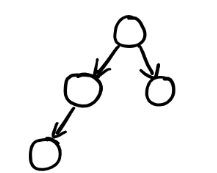
\includegraphics[width=.35\textwidth]{微信图片_20191124100458.png}
    \caption{基本概率图模型}
    
\end{figure}
对于一个箭头$\longrightarrow$来说,箭头所在的方向称为Head,另一端被称为Tail。

\subsection{Tail to Tail结构}
Tail to Tail的模型结构图,如下图所示,由于b节点在a节点和c节点的Tail部分,所以被我们称为Tail to Tail结构。
\begin{figure}[H]
    \centering
    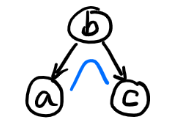
\includegraphics[width=.35\textwidth]{微信图片_20191124101337.png}
    \caption{Tail to Tail结构示意图}
    
\end{figure}

我们使用因子分析来计算联合概率可以得到:
\begin{equation}
    p(a,b,c) = p(b)p(a|b)p(c|b)
\end{equation}

使用链式法则,同样我们也可以得到:
\begin{equation}
    p(a,b,c) = p(b)p(a|b)p(c|b,a)
\end{equation}

对比一下公式(3)和公式(4),我们可以对比得到:
\begin{equation}
    p(c|b)=p(c|b,a)
\end{equation}

实际上,这里就已经就可以看出$a\bot c$了,因为$a$的条件增不增加都不会改变$c$的概率,所以$a$和$c$之间是相互独立的。可能有的同学还是觉得不好理解,那么我们做进一步的分析:
\begin{gather}
    p(c|b)p(a|b) = p(c|b,a)p(a|b) = p(a,c|b) \\ 
    \Rightarrow p(c|b)p(a|b) = p(a,c|b)
\end{gather}
这样,我们就可以看得很明白了。这就是条件独立性,在a的条件下,b和c是独立的。实际在概率图中就已经蕴含这个分解了,只看图我们就可以看到这个性质了,这就是图的直观性,条件独立性和图是一样的。那么$a\bot c$可以被我们看为:给定$b$的情况下,如果$b$被观测到,那么$a$和$c$之间是阻塞的,也就是相互独立。

\subsection{Head to Tail结构}
\begin{figure}[H]
    \centering
    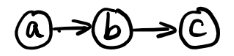
\includegraphics[width=.35\textwidth]{微信图片_20191124103526.png}
    \caption{Head to Tail结构示意图}
    
\end{figure}

其实,和Head to Head结构的分析基本是上一模一样的,我们可以得到$a\bot c|b$。也就是给定$b$的条件下,$a$和$c$之间是条件独立的。也就是$b$被观测的条件下,路径被阻塞。

\subsection{Head to Head结构}
\begin{figure}[H]
    \centering
    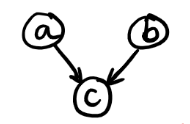
\includegraphics[width=.35\textwidth]{微信图片_20191124104553.png}
    \caption{Head to Head结构示意图}
    
\end{figure}
在默认情况下$a\bot b$,也就是若$c$被观测,$a$和$b$之间是有关系的。我们可以推导一下默认情况。
\begin{equation}
    \begin{split}
        p(a,b,c) = & p(a)p(b)p(c|a,b) \\
        = & p(a)p(b|a)p(c|a,b)
    \end{split}
\end{equation}

我们可以得出$p(b)=p(b|a)$,也就是$a\bot b$。








\end{document}